\documentclass[a4paper,twoside,DIV15,BCOR12mm]{scrbook}

\usepackage{mathe}
\usepackage{saetze-baeuerle}
\usepackage{faktor}
\usepackage{enumerate}
\usepackage{tikz}

\newcommand{\cF}{\mathcal{F}}

\author{Die Mitarbeiter von \url{http://mitschriebwiki.nomeata.de/}}
\title{Stochasitsche Prozesse}
\makeindex

\begin{document}
\maketitle
 

\renewcommand{\thechapter}{\Roman{chapter}}
%\chapter{Inhaltsverzeichnis}
\stepcounter{chapter}
%\renewcommand{\tocname}{bla}
\addcontentsline{toc}{chapter}{\protect\numberline {\thechapter}Inhaltsverzeichnis}
\tableofcontents

 % Vorwort

\chapter{Vorwort}
%\addcontentsline{toc}{chapter}{Vorwort}

\section*{Über dieses Skriptum}
Dies ist ein Mitschrieb der Vorlesung \glqq Stochastische Prozesse\grqq\ von Prof. Dr. Bäuerle im
Sommersemester 08 an der Universität Karlsruhe (TH).
Die Mitschriebe der Vorlesung werden mit ausdrücklicher Genehmigung von Prof Dr. Bäuerle hier veröffentlicht,
Prof. Dr. Bäuerle ist für  den Inhalt nicht verantwortlich.
\section*{Wer}
Gestartet wurde das Projekt von Joachim Breitner.


\section*{Wo}
Alle Kapitel inklusive \LaTeX-Quellen können unter \url{http://mitschriebwiki.nomeata.de} abgerufen werden.
Dort ist ein von Joachim Breitner programmiertes \emph{Wiki}, basierend auf \url{http://latexki.nomeata.de} installiert. 
Das heißt, jeder kann Fehler nachbessern und sich an der Entwicklung
beteiligen. Auf Wunsch ist auch ein Zugang über \emph{Subversion} möglich.

\setcounter{chapter}{0}
%\renewcommand{\thesection}{{\rm\bfseries §}\arabic{section}}
\renewcommand{\thechapter}{\arabic{chapter}}

\chapter{Markov-Ketten mit diskretem Zeitparameter}

\section{Elementare Eigenschaften von Markov-Ketten}

Gegeben sei eine Folge von Zufallsvariablen $(X_n)$ auf dem Wahrscheinlichkeitsraum $(\Omega, \cF, P)$ mit $X_n:\Omega \to S$ wobei $S$ nicht leer, und endlich oder abzählbar unendlich ist.

\begin{definition}
Eine $S\times S$-Matrix $P=(p_{ij})$ heißt \emph{stochastische Matrix}\index{stochastische Matrix}, falls $p_{ij}>0$ ist und für alle $i\in S$ die Zeilensumme $\sum_{j\in S} p_{ij} = 1$ ist.
\end{definition}

\begin{definition}
Sei $P$ eine stochastische Matrix. Eine (endliche oder unendliche) Folge $X_0, X_1, X_2,\ldots$ von $S$-wertigen Zufallsvariablen heißt (homogene\footnote{kurz für zeit-homogen. Die Übergangswahrscheinlichkeiten hängen nicht vom aktuellen Zeitpunkt ab.}) \emph{Markov-Kette}\index{Markov-Kette} mit Übergangsmatrix $P$, falls für alle $n\in \MdN$\footnote{Hier ist $\MdN=1,2,\ldots$} und für alle Zustände $i_k\in S$ mit 
\[
P(X_0=i_0,\ldots,X_n=i_n) >0
\]
gilt
\[
P(X_{n+1} = i_{n+1} \mid X_0 = i_0, \ldots, X_n=i_n) = 
P(X_{n+1} = i_{n+1} \mid X_n=i_n) = p_{i_n i_{n+1}}.
\]

Die $p_{ij}$ heißen Übergangswahrscheinlichkeiten und die \emph{Startverteilung} $\nu$ der Kette ist definiert durch $\nu(i)=P(X_0=i)$ für $i\in S$.
\end{definition}

\begin{bemerkung}
Jede Folge von unabhängigen Zufallsvariablen ist eine Markov-Kette.
\end{bemerkung}

\begin{satz}[Eigenschaften von Markov-Ketten]
$(X_n)$ ist genau dann eine Markovkette mit Übergangsmatrix $P$, falls gilt:
\[
P(X_k = i_k,\, 0\le k\le n) = P(X_0 = i_0)\prod_{k=0}^{n-1} p_{i_k i_{k+1}} \quad \forall n\in \MdN_0 \ \forall i_k\in S
\]
genau dann wenn gilt:
\[
P(X_k = i_k,\, 1\le k\le n \mid X_0=i_0) = \prod_{k=0}^{n-1} p_{i_k i_{k+1}} \quad \forall n\in \MdN_0 \ \forall i_k\in S\text{ mit $P(X_0=i_0)>0$}
\]
genau dann wenn gilt:
\[
P(X_k = i_k,\,m\le k\le m+n) = \prod_{k=m}^{m+n-1} p_{i_k i_{k+1}} \quad \forall m,n\in \MdN_0 \ \forall i_k\in S
\]
\end{satz}

\begin{beweis}
Zur ersten Äquivalenz. Sei $A_k \da [X_k=i_k]$, $k\in\MdN_0$.

„$\Longrightarrow$“ Induktion über $n$: $n=0$ $\checkmark$, $n\curvearrowright n+1:$ 
\begin{align*}
P(A_0A_1\ldots A_nA_{n+1}) &= P(A_0\ldots A_n)\cdot P(A_{n+1}\mid A_0\ldots A_n) \\
&= P(A_0\ldots A_n)\cdot p_{i_ni_{n+1}} && \text{(Markov-Eigenschaft)}\\
&= P(X_0=i_0)\prod_{k=0}^n p_{i_ki_{k+1}} && \text{(I.V.)}
\end{align*}

„$\Longleftarrow$“ 
\begin{align*}
P(A_{n+1}\mid A_0\ldots A_n) &= \frac{P(A_0\ldots A_nA_{n+1})}{P(A_0\ldots A_n)} \\
&= p_{i_ni_{n+1}} && \text{(Vor.)}
\end{align*}
Die weiteren Äquivalenzen sind ähnlich zu beweisen.
\end{beweis}

\paragraph{Konstruktion einer Markov-Kette.} Seien $(Y_n)$ Zufallsvariablen, unabhängig und identisch gleichverteilt (u.i.v.), in $Z$. Weiter ist $g:S\times Z\to S$ eine messbare Abbildung. Definiere die Folge $(X_n)$ mit 
\[X_0=c\in S, \quad X_n = g(X_{n-1},Y_n).\]
Die so konstruierte Folge $(X_n)$ ist eine Markov-Kette mit Werten in $S$ und Übergangsmatrix $P=(p_{ij})$ mit $p_{ij} = P(g(i,X_n),j)$.

\begin{beweis}
Die Variablen $X_0,\ldots,X_n$ hängen nur von $X_0,Y_1,\ldots Y_n$ ab, sind also unabhängig von $Y_{n+1}$.
\begin{align*}
P(X_{n+1} = i_{n+1} \mid X_k = i_k, 0\le k\le n) 
&= \frac{P(X_k = i_k,\, 0\le k\le n+1)}{P(X_k = i_k,\, 0\le k\le n)} \\
&= \frac{P(X_k = i_k,\, 0\le k\le n,\, g(i_n,Y_{n+1})=i_{n+1})}{P(X_k = i_k,\, 0\le k\le n)} \\
&= \frac{P(X_k = i_k,\, 0\le k\le n)\cdot P(g(i_n,Y_{n+1})=i_{n+1})}{P(X_k = i_k,\, 0\le k\le n)} \\
&= P(g(i_n,Y_{n+1})=i_{n+1}) \\
&= \frac{P(g(i_n,Y_{n+1})=i_{n+1})\cdot P(X_n=i_n)}{P(X_n =i_n)} \\
&= \frac{P(g(i_n,Y_{n+1})=i_{n+1}, X_n=i_n)}{P(X_n =i_n)} \\
&= P(g(i_n,Y_{n+1})=i_{n+1}\mid X_n=i_n) \\
&= P(X_{n+1} = i_{n+1} \mid X_n=i_n)
\end{align*}
\end{beweis}

\begin{bemerkung}
Umgekehrt kann zu jeder stochastischen Matrix $P$ eine Markovkette $(X_n)$ konstruiert werden mit $X_n=g(X_{n-1},Y_n)$, wobei $(Y_n)$ u.i.v. und o.B.d.A $Y_n \sim U[0,1]$.
\end{bemerkung}

\begin{beispiel}[Lagerhaltung]
Sei $Y_n$ die Nachfrage nach einem gelagerten Produkt im Zeitintervall $(n-1,n]$. $(Y_n)$ sei u.i.v. und $Y_n\in \MdN_0$. Die Auffüll-Politik sei eine $(z,Z)$-Politik mit $z\le Z$, $z,Z\in \MdN$, die wie folgt funktiert: Falls der der Lagerbestand zur Zeit $n\le z$ ist, dann fülle auf $Z$ auf, sonst tue nichts.

Sei $X_n$ der Lagerbestand zum Zeitpunkt $n$, $S=\MdN_0$. Es gilt
\[
X_n =
\begin{cases}
(Z - Y_n)^+, & X_{n-1} \le z \\
(X_{n+1} - Y_n)^+, & X_{n-1} > z
\end{cases}
\]
Also ist $(X_n)$ eine Markov-Kette mit Übergangsmatrix $P=(p_{ij})$ und
\[
p_{ij} = 
\begin{cases}
P( (Z-Y_n)^+ = j), & i\le z \\
P( (i-Y_n)^+ = j), & i > z
\end{cases}
\]
\end{beispiel}

\begin{beispiel}[Ruinspiel]
Zwei Spieler mit Startkapital $B\in\MdN$ Euro spielen in Runden um jeweils einen Euro, etwa mit einem Münzwurf. Spieler I gewinnt dabei mit Wahrscheinlichkeit $p$. Sei $Y_n = 1$, falls Spieler I die $n$-te Runde gewinnt, und $Y_n= -1$, falls er die $n$-Runde verliert. Wir nehmen an, dass $Y_n$ u.i.v. ist.

Wir interessieren uns für das Kapital $X_n$ von Spieler I nach der $n$-ten Runde. Damit ist der Zustandsraum $S=\{0,1,\ldots,2B\}$.

Es gilt $X_0 = B$ und
\[
X_n = 
\begin{cases}
2B, &X_{n-1} = 2B \\
X_{n-1} + Y_n, & 0 < X_{n-1} < 2B \\
0, &X_{n-1} = 0.
\end{cases}
\]
Es folgt aus der Konstruktion direkt dass $(X_n)$ eine Markov-Kette ist mit Übergangsmatrix $P=(p_{ij})$, und
$p_{00} = p_{2B,2B} = 1$ sowie
\[
p_{ij} = 
\begin{cases}
p, &j=i+1\\
1-p, &j=i-1 
\end{cases}\text{ für } 0<i<2B.
\]
% Wer lust hat: Hier skizze mit Übergangswahrscheinlichkeiten.
\begin{center}
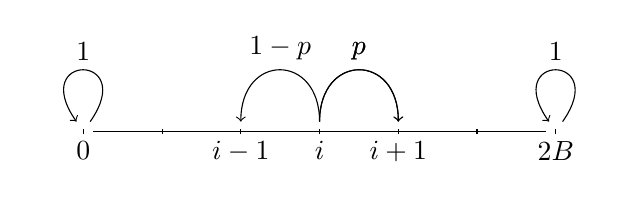
\begin{tikzpicture}
\foreach \x in {0,1,2,3,4,5,6}
	\draw (\x cm,-1pt) -- (\x cm, 1pt);
\node (null) at (0,0) {}; \draw (null) node[anchor=north] {$0$};
\node (a) at (2,0) {}; \draw (a) node [anchor=north] {$i-1$};
\node (b) at (3,0) {}; \draw (b) node [anchor=north] {$i$};
\node (c) at (4,0) {}; \draw (c) node [anchor=north] {$i+1$};
\node (zb) at (6,0) {}; \draw (zb) node [anchor=north] {$2B$};
\draw (null) -- (zb);
\draw [->] (b) .. controls +(up:1cm) and +(up:1cm) .. node [anchor=south] {$1-p$}  (a);
\draw [->] (b) .. controls +(up:1cm) and +(up:1cm) .. node [anchor=south] {$p$}  (c);
\draw [->] (b) .. controls +(up:1cm) and +(up:1cm) .. node [anchor=south] {$p$}  (c);
\draw [->] (null) .. controls +(0.7,1) and +(-0.7,1) .. node [anchor=south] {$1$}  (null);
\draw [->] (zb) .. controls +(0.7,1) and +(-0.7,1) .. node [anchor=south] {$1$}  (zb);
\end{tikzpicture}
\end{center}
\end{beispiel}

\begin{beispiel}[Wartesystem]
Zu jedem Zeitpunkt $n=0,1,\ldots$ können maximal $m$ Kunden bedient werden. $Y_n$ sei die Anzahl der zufällig im Zeitintervall $(n-1,n]$ eintreffenden Kunden und sei u.i.v.

Sei $X_n$ die Anzahl der zur Zeit $n$ wartenden Kunden, $S=\MdN_0$. Es gilt $X_0 = C$ und $X_n = (X_{n-1}-m)^+ + Y_n$. Also ist $(X_n)$ eine Markov-Kette mit Übergangsmatrix $P=(p_{ij})$ und $p_{ij} = P(Y_n = j-(i-m)^+)$, $i,j\in \MdN_0$.
\end{beispiel}

\begin{definition}
Sei $P$ eine stochastische $S\times S$-Matrix. Dann heißen die Elemente $p_{ij}^{(n)}$ von $P^n$ die $n$-Schritt-Übergangswahrscheinlichkeiten zu $P$. Wir definieren $P^0=E$, also $p_{ij}= \delta_{ij}$.
\end{definition}

\begin{satz}
Sei $(X_n)$ eine Markov-Kette mit Übergangsmatrix $P$. Dann gilt:
\begin{enumerate}[a)]
\item $P(X_{n+m} = j\mid X_m = i) = p_{ij}^{(n)}$ für alle $i,j\in S$, $m,n\in\MdN_0$ mit $P(X_m=1)>0$.
\item $P(X_n = j) = \sum_{i\in S} P(X_0=i)p_{ij}^{(n)}$, $j\in S$, $n\in\MdN$.
\end{enumerate}
\end{satz}

\begin{beweis}
\begin{enumerate}[a)]
\item 
\begin{align*}
P(X_{n+m} =i_{n+m} , X_m=i_m) &= \sum_{i_{m+1},\ldots,i_{n+m+1}} P(X_m = i_m) \prod_{k=m}^{m+n+1} p_{i_ki_{k+1}} \\
&= P(X_m = i_m) p_{i_mi_{m+n}}^{(n)}
\end{align*}
\item 
\begin{align*}
P(X_n=j) &= \sum_{i\in S} P(X_n=j, X_0=i) \\
&= \sum_{i\in S} P(X_n = j \mid X_0 = i)\cdot P(X_0 = i) \\
&= \sum_{i\in S} P(X_0) p_{ij}^{(n)}
\end{align*}
\end{enumerate}
\end{beweis}

\begin{bemerkung}
\begin{enumerate}[(i)]
\item Wegen $p^{n+m}  = p^n \cdot p^m$ gilt: 
\[
p_{ij}^{(n+m)}  = \sum_{k\in S} p_{ij}^{(n)}p_{kj}^{(m)} \text{ für } i,j\in S
\]
Dies ist die „Chapman-Kologomorov-Gleichung“\index{Chapman-Kologomorov-Gleichung}.
\item Ist $X_0 \sim \nu$, so gilt $X_n \sim \nu\cdot P^n$.
\end{enumerate}
\end{bemerkung}

\begin{satz}[Existenzssatz für Markov-Ketten]
Sei $\nu$ ein Wahrscheinlichkeitsmaß auf $S$ und $P$ eine stochastische $S\times S$-Matrix. Sei $X_n$ die $n$-te Projektion auf $\Omega \da S^{\MdN_0}$, also $X_n : \Omega\to s$, $n\in\MdN_0$ mit $X_n(\omega) = X_n( (i_0,i_1,\ldots) ) = i_n$.

Dann existiert ein Wahrscheinlichkeitsmaß $P$ auf $\cF = \oplus_{n=0}^\infty \mathcal P (S)$, so dass $(X_n)$ eine Markov-Kette mit Übergangsmatrix $P$ und Startverteilung $\nu$ ist, d.h:
\begin{itemize}
\item $P(X_0 = i_0)= \nu(i_0)$, $i_0\in S$
\item $P(X_{n+1} = j \mid X_n= j) = p_{ij}$, $i,j\in S$, $P(X_n=i)>0$.
\end{itemize}
\end{satz}

\begin{beweis}
Staz von Ionescu-Tulcea über die Fortsetzung von Maßen und die Existenz zufälliger Folgen.
\end{beweis}

\section{Klassifikation von Zuständen, Rekurrenz und Transienz}

In diesem Paragraphen widmen wir uns Fragestellungen wie diesen:
Welche Zustände in $S$ werden von der Markov-Kette mit Sicherheit besucht und welche nicht? Wenn sie besucht werden, wie oft? 

\begin{definition}
Sei $(X_n)$ eine Markov-Kette mit Übergangsmatrix $P=(p_{ij})$.
\begin{enumerate}[a)]
\item $i\in S$ \emph{führt nach} $j\in S$ (kurz $i\rightsquigarrow j$)\index{$\rightsquigarrow$}, falls es ein $n\in \MdN$ gibt mit $p_{ij}^{(n)}>0$.

\item $i\in S$ \emph{kommuniziert} mit $j\in S$ (kurz $i\leftrightarrow j)$\index{$\leftrightarrow$} falls sowohl $i\rightsquigarrow j$ als auch $j\rightsquigarrow i$ gilt.
\end{enumerate}
\end{definition}

\begin{bemerkung}
Für $i,j\in S$ sei $i\sim j$ definiert als $(i\leftrightarrow j) \vee (i=j)$. Diese Relation ist eine Äquivalentrelation auf $S$, da sie reflexiv, symmetrisch und transitiv ist.

Dies liefert uns eine Partition von $S$ mit den Äquivalenzklassen $K(i) \da \{j\in S \mid i\sim j\}$. Die Äquivalenzklasse $K(i)$ von $i$ enthält $i$ selbst und die mit $i$ kommunizierenden Zustände.
\end{bemerkung}

\begin{definition}
Sei $(X_n)$ eine Markov-Kette mit Übergangsmatrix $P=(p_{ij})$.
\begin{enumerate}[a)]
\item $J\subset S$ heißt \emph{abgeschlossen}\index{abgeschlossene Zustandsmenge}, wenn es keine zwei Zustände $i\in J$ und $i\in S\setminus J$ gibt mit $j\rightsquigarrow i$.
\item Die Markov-Kette $(X_n)$ beziehungsweise die Übergangsmatrix $P$ heißen \emph{irreduzibel}\index{irreduzibel}, falls $S$ nur aus einer Klasse besteht, also für alle $i,j\in S$, $i\ne j$, gilt $i\leftrightarrow j$.
\end{enumerate}
\end{definition}

\begin{beispiel}
\emph{Skizze, hier ausgelassen}
\end{beispiel}

\begin{beispiel}[Ruinspiel]
$\mbox{}$
\begin{center}
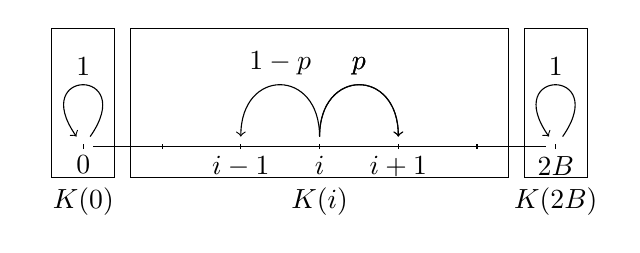
\begin{tikzpicture}
\foreach \x in {0,1,2,3,4,5,6}
	\draw (\x cm,-1pt) -- (\x cm, 1pt);
\node (null) at (0,0) {}; \draw (null) node[anchor=north] {$0$};
\node (a) at (2,0) {}; \draw (a) node [anchor=north] {$i-1$};
\node (b) at (3,0) {}; \draw (b) node [anchor=north] {$i$};
\node (c) at (4,0) {}; \draw (c) node [anchor=north] {$i+1$};
\node (zb) at (6,0) {}; \draw (zb) node [anchor=north] {$2B$};
\draw (null) -- (zb);
\draw [->] (b) .. controls +(up:1cm) and +(up:1cm) .. node [anchor=south] {$1-p$}  (a);
\draw [->] (b) .. controls +(up:1cm) and +(up:1cm) .. node [anchor=south] {$p$}  (c);
\draw [->] (b) .. controls +(up:1cm) and +(up:1cm) .. node [anchor=south] {$p$}  (c);
\draw [->] (null) .. controls +(0.7,1) and +(-0.7,1) .. node [anchor=south] {$1$}  (null);
\draw [->] (zb) .. controls +(0.7,1) and +(-0.7,1) .. node [anchor=south] {$1$}  (zb);
\draw (-0.4,-0.4) rectangle (0.4,1.5);
\draw (0,-0.4) node [anchor=north] {$K(0)$};
\draw (0.6,-0.4) rectangle (5.4,1.5);
\draw (3,-0.4) node [anchor=north] {$K(i)$};
\draw (5.6,-0.4) rectangle (6.4,1.5);
\draw (6,-0.4) node [anchor=north] {$K(2B)$};
\end{tikzpicture}
\end{center}

\end{beispiel}

\chapter{Satz um Satz (hüpft der Has)}
\listtheorems{satz,wichtigedefinition}

\renewcommand{\indexname}{Stichwortverzeichnis}
\addtocounter{chapter}{1}
\addcontentsline{toc}{chapter}{\protect\numberline {\thechapter}Stichwortverzeichnis}
\printindex
\end{document}
